% GNUPLOT: LaTeX picture with Postscript
\begingroup
\newcommand{\ft}[0]{\footnotesize}
  \makeatletter
  \providecommand\color[2][]{%
    \GenericError{(gnuplot) \space\space\space\@spaces}{%
      Package color not loaded in conjunction with
      terminal option `colourtext'%
    }{See the gnuplot documentation for explanation.%
    }{Either use 'blacktext' in gnuplot or load the package
      color.sty in LaTeX.}%
    \renewcommand\color[2][]{}%
  }%
  \providecommand\includegraphics[2][]{%
    \GenericError{(gnuplot) \space\space\space\@spaces}{%
      Package graphicx or graphics not loaded%
    }{See the gnuplot documentation for explanation.%
    }{The gnuplot epslatex terminal needs graphicx.sty or graphics.sty.}%
    \renewcommand\includegraphics[2][]{}%
  }%
  \providecommand\rotatebox[2]{#2}%
  \@ifundefined{ifGPcolor}{%
    \newif\ifGPcolor
    \GPcolortrue
  }{}%
  \@ifundefined{ifGPblacktext}{%
    \newif\ifGPblacktext
    \GPblacktextfalse
  }{}%
  % define a \g@addto@macro without @ in the name:
  \let\gplgaddtomacro\g@addto@macro
  % define empty templates for all commands taking text:
  \gdef\gplbacktext{}%
  \gdef\gplfronttext{}%
  \makeatother
  \ifGPblacktext
    % no textcolor at all
    \def\colorrgb#1{}%
    \def\colorgray#1{}%
  \else
    % gray or color?
    \ifGPcolor
      \def\colorrgb#1{\color[rgb]{#1}}%
      \def\colorgray#1{\color[gray]{#1}}%
      \expandafter\def\csname LTw\endcsname{\color{white}}%
      \expandafter\def\csname LTb\endcsname{\color{black}}%
      \expandafter\def\csname LTa\endcsname{\color{black}}%
      \expandafter\def\csname LT0\endcsname{\color[rgb]{1,0,0}}%
      \expandafter\def\csname LT1\endcsname{\color[rgb]{0,1,0}}%
      \expandafter\def\csname LT2\endcsname{\color[rgb]{0,0,1}}%
      \expandafter\def\csname LT3\endcsname{\color[rgb]{1,0,1}}%
      \expandafter\def\csname LT4\endcsname{\color[rgb]{0,1,1}}%
      \expandafter\def\csname LT5\endcsname{\color[rgb]{1,1,0}}%
      \expandafter\def\csname LT6\endcsname{\color[rgb]{0,0,0}}%
      \expandafter\def\csname LT7\endcsname{\color[rgb]{1,0.3,0}}%
      \expandafter\def\csname LT8\endcsname{\color[rgb]{0.5,0.5,0.5}}%
    \else
      % gray
      \def\colorrgb#1{\color{black}}%
      \def\colorgray#1{\color[gray]{#1}}%
      \expandafter\def\csname LTw\endcsname{\color{white}}%
      \expandafter\def\csname LTb\endcsname{\color{black}}%
      \expandafter\def\csname LTa\endcsname{\color{black}}%
      \expandafter\def\csname LT0\endcsname{\color{black}}%
      \expandafter\def\csname LT1\endcsname{\color{black}}%
      \expandafter\def\csname LT2\endcsname{\color{black}}%
      \expandafter\def\csname LT3\endcsname{\color{black}}%
      \expandafter\def\csname LT4\endcsname{\color{black}}%
      \expandafter\def\csname LT5\endcsname{\color{black}}%
      \expandafter\def\csname LT6\endcsname{\color{black}}%
      \expandafter\def\csname LT7\endcsname{\color{black}}%
      \expandafter\def\csname LT8\endcsname{\color{black}}%
    \fi
  \fi
  \setlength{\unitlength}{0.0500bp}%
  \begin{picture}(8502.00,5668.00)%
    \gplgaddtomacro\gplbacktext{%
      \colorrgb{0.50,0.50,0.50}%
      \put(814,751){\makebox(0,0)[r]{\strut{} 0}}%
      \colorrgb{0.50,0.50,0.50}%
      \put(814,1216){\makebox(0,0)[r]{\strut{} 5}}%
      \colorrgb{0.50,0.50,0.50}%
      \put(814,1681){\makebox(0,0)[r]{\strut{} 10}}%
      \colorrgb{0.50,0.50,0.50}%
      \put(814,2147){\makebox(0,0)[r]{\strut{} 15}}%
      \colorrgb{0.50,0.50,0.50}%
      \put(814,2612){\makebox(0,0)[r]{\strut{} 20}}%
      \colorrgb{0.50,0.50,0.50}%
      \put(814,3077){\makebox(0,0)[r]{\strut{} 25}}%
      \colorrgb{0.50,0.50,0.50}%
      \put(814,3542){\makebox(0,0)[r]{\strut{} 30}}%
      \colorrgb{0.50,0.50,0.50}%
      \put(814,4007){\makebox(0,0)[r]{\strut{} 35}}%
      \colorrgb{0.50,0.50,0.50}%
      \put(814,4473){\makebox(0,0)[r]{\strut{} 40}}%
      \colorrgb{0.50,0.50,0.50}%
      \put(814,4938){\makebox(0,0)[r]{\strut{} 45}}%
      \colorrgb{0.50,0.50,0.50}%
      \put(814,5403){\makebox(0,0)[r]{\strut{} 50}}%
      \colorrgb{0.50,0.50,0.50}%
      \put(993,484){\makebox(0,0){\strut{}1}}%
      \colorrgb{0.50,0.50,0.50}%
      \put(1302,484){\makebox(0,0){\strut{}2}}%
      \colorrgb{0.50,0.50,0.50}%
      \put(1611,484){\makebox(0,0){\strut{}3}}%
      \colorrgb{0.50,0.50,0.50}%
      \put(1921,484){\makebox(0,0){\strut{}4}}%
      \colorrgb{0.50,0.50,0.50}%
      \put(2230,484){\makebox(0,0){\strut{}5}}%
      \colorrgb{0.50,0.50,0.50}%
      \put(2539,484){\makebox(0,0){\strut{}6}}%
      \colorrgb{0.50,0.50,0.50}%
      \put(2848,484){\makebox(0,0){\strut{}7}}%
      \colorrgb{0.50,0.50,0.50}%
      \put(3158,484){\makebox(0,0){\strut{}8}}%
      \colorrgb{0.50,0.50,0.50}%
      \put(3467,484){\makebox(0,0){\strut{}9}}%
      \colorrgb{0.50,0.50,0.50}%
      \put(3776,484){\makebox(0,0){\strut{}10}}%
      \colorrgb{0.50,0.50,0.50}%
      \put(4085,484){\makebox(0,0){\strut{}11}}%
      \colorrgb{0.50,0.50,0.50}%
      \put(4394,484){\makebox(0,0){\strut{}12}}%
      \colorrgb{0.50,0.50,0.50}%
      \put(4704,484){\makebox(0,0){\strut{}13}}%
      \colorrgb{0.50,0.50,0.50}%
      \put(5013,484){\makebox(0,0){\strut{}14}}%
      \colorrgb{0.50,0.50,0.50}%
      \put(5322,484){\makebox(0,0){\strut{}15}}%
      \colorrgb{0.50,0.50,0.50}%
      \put(5631,484){\makebox(0,0){\strut{}16}}%
      \colorrgb{0.50,0.50,0.50}%
      \put(5940,484){\makebox(0,0){\strut{}17}}%
      \colorrgb{0.50,0.50,0.50}%
      \put(6250,484){\makebox(0,0){\strut{}18}}%
      \colorrgb{0.50,0.50,0.50}%
      \put(6559,484){\makebox(0,0){\strut{}19}}%
      \colorrgb{0.50,0.50,0.50}%
      \put(6868,484){\makebox(0,0){\strut{}20}}%
      \colorrgb{0.50,0.50,0.50}%
      \put(7177,484){\makebox(0,0){\strut{}21}}%
      \colorrgb{0.50,0.50,0.50}%
      \put(7487,484){\makebox(0,0){\strut{}22}}%
      \colorrgb{0.50,0.50,0.50}%
      \put(7796,484){\makebox(0,0){\strut{}23}}%
      \colorrgb{0.50,0.50,0.50}%
      \put(8105,484){\makebox(0,0){\strut{}24}}%
      \csname LTb\endcsname%
      \put(176,3077){\rotatebox{-270}{\makebox(0,0){\strut{}Przyspieszenie S}}}%
      \put(4549,154){\makebox(0,0){\strut{}Liczba wątków}}%
    }%
    \gplgaddtomacro\gplfronttext{%
      \csname LTb\endcsname%
      \put(7118,5230){\makebox(0,0)[r]{\strut{}OMP parfor}}%
      \csname LTb\endcsname%
      \put(7118,5010){\makebox(0,0)[r]{\strut{}MKL DGEMM}}%
      \csname LTb\endcsname%
      \put(7118,4790){\makebox(0,0)[r]{\strut{}Naiwny}}%
    }%
    \gplbacktext
    \put(0,0){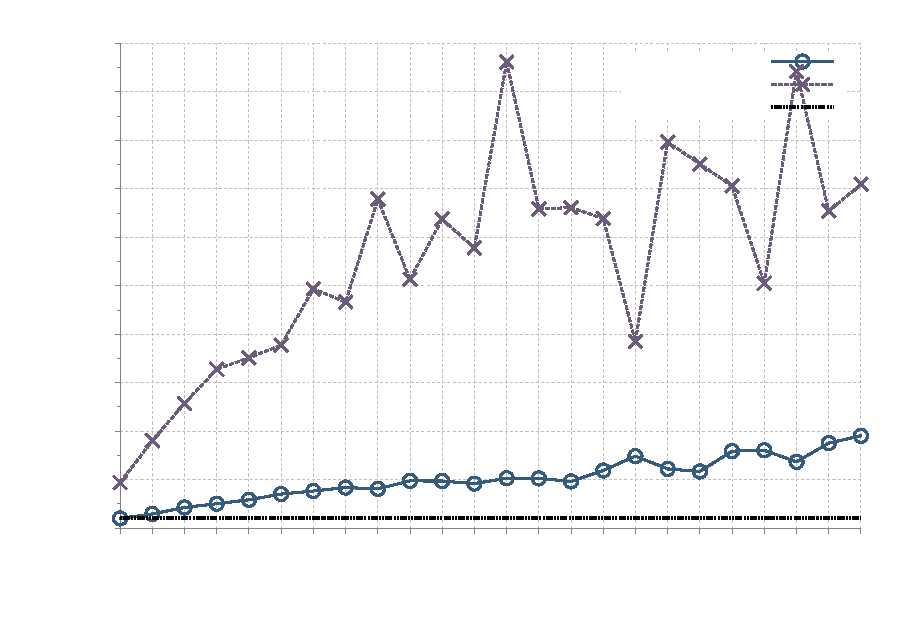
\includegraphics{mono}}%
    \gplfronttext
  \end{picture}%
\endgroup
